En esta sección se detallarán los casos de uso pertenecientes al subsistema de gestión de noticias. La figura \ref{fig:casos_uso_subsistema_noticias} muestra el diagrama de casos de uso de dicho subsistema.

\begin{figure}[h]
\centering
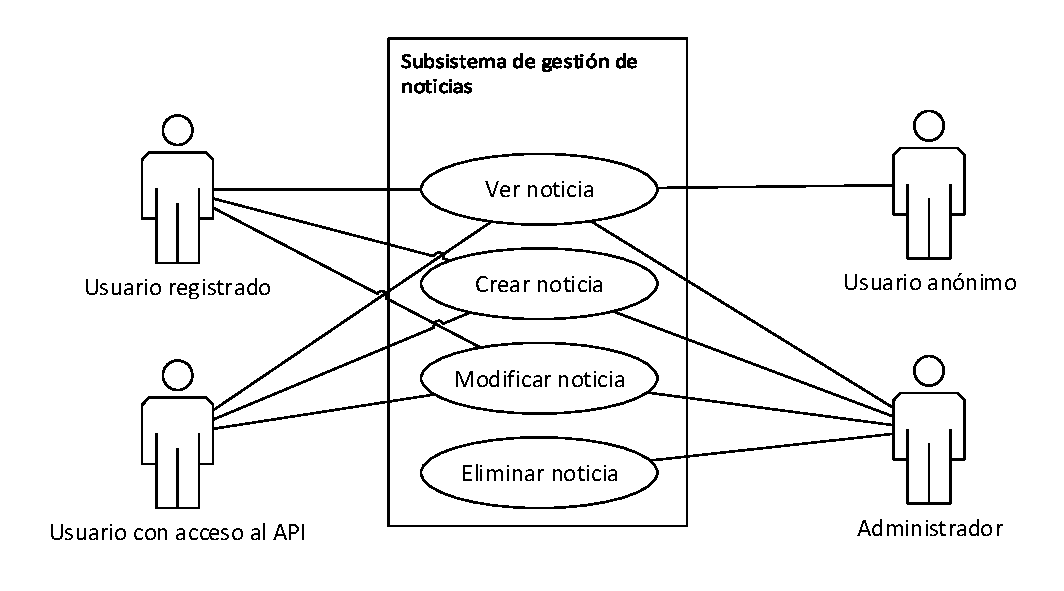
\includegraphics[width=\textwidth]{casos_uso/diagrama_casos_uso_noticias}
\caption{Diagrama de casos de uso del subsistema de gestión de noticias}
\label{fig:casos_uso_subsistema_noticias}
\end{figure}


\subsubsection{Caso de uso ``ver noticia''}
\begin{description}
\item[Descripción] Un usuario quiere ver el contenido de una noticia.
\item[Actores] Cualquier usuario registrado o no en el sistema.
\item[Escenario principal] 	\hfill
							\begin{enumerate}
							\item El usuario pulsa en el botón que carga la vista de las noticias.
							\item Una vez en la vista de noticias pulsa en el título de la noticia que quiere ver en detalle.
							\item El sistema carga la vista de la noticia mostrando todos sus detalles.
							\end{enumerate}
\end{description}


\subsubsection{Caso de uso ``crear noticia''}
\begin{description}
\item[Descripción]  Un usuario quiere añadir una nueva noticia al sistema.
\item[Actores]  Administrador, usuario registrado o usuario con capacidad de acceso al API.
\item[Precondiciones] Haber iniciado sesión en el sistema.
\item[Escenario principal]  \hfill
							\begin{enumerate}
							\item El usuario pulsa en el botón que carga la vista de las noticias.
							\item Una vez en la vista de las noticias pulsa el botón correspondiente para crear una noticia nueva.
							\item Rellena el formulario con los datos requeridos.
							\item Si lo desea también rellena la información opcional del formulario.
							\item El usuario pulsa el botón guardar.
							\item El sistema crea la nueva noticia.
							\end{enumerate}
\item[Escenario alternativo 1] No se han rellenado todos los campos requeridos.
							\begin{enumerate}
							\item El usuario no ha rellenado todos los campos requeridos para crear una nueva noticia.
							\item El sistema notificará al usuario de su error y no creará la nueva noticia.
							\item Se continuará desde el punto 3 del escenario principal.
							\end{enumerate}
\end{description}


\subsubsection{Caso de uso ``modificar noticia''}
\begin{description}
\item[Descripción]  Un usuario quiere modificar una noticia del sistema.
\item[Actores]  Administrador, usuario registrado o usuario con capacidad de acceso al API.
\item[Precondiciones]  Haber iniciado sesión en el sistema.
\item[Escenario principal]	\hfill
							\begin{enumerate}
							\item El usuario accede a la vista de las noticias.
							\item Una vez en la vista de noticias localiza la noticia que quiere modificar.
							\item Cuando ha accedido a la noticia pulsa el botón correspondiente para modificar su contenido.
							\item Rellena toda la información requerida en el formulario.
							\item Si lo desea también rellena la información opcional del formulario.
							\item El usuario pulsa el botón guardar.
							\item El sistema actualiza la información de la noticia editada.
							\end{enumerate}
\item[Escenario alternativo 1] No se han rellenado todos los campos requeridos.
							\begin{enumerate}
							\item El usuario no ha rellenado todos los campos requeridos para modificar la noticia.
							\item El sistema notificará al usuario de su error y no modificará los datos de la noticia.
							\item Se continuará desde el punto 4 del escenario principal.
							\end{enumerate}
\end{description}


\subsubsection{Caso de uso ``eliminar noticia''}
\begin{description}
\item[Descripción]  Un administrador quiere eliminar una noticia del sistema.
\item[Actores]  El administrador del sistema.
\item[Precondiciones]  Haber iniciado sesión en el sistema.
\item[Escenario principal]	\hfill
							\begin{enumerate}
							\item El administrador accede a la vista de noticias.
							\item Accede a la noticia que desea eliminar.
							\item Una vez en la vista de la noticia pulsa el botón correspondiente para su eliminación.
							\item La noticia será eliminada del sistema.
							\end{enumerate}
\end{description}